\documentclass[11pt]{article}

\usepackage[margin=1in]{geometry}
\usepackage[utf8]{inputenc}
\usepackage[T1]{fontenc}
\usepackage{lmodern}
\usepackage{microtype}
\usepackage{graphicx}
\usepackage{booktabs}
\usepackage{amsmath, amssymb}
\usepackage{array}
\usepackage{multirow}
\usepackage{float}
\usepackage[hidelinks]{hyperref}
\usepackage[numbers,sort&compress]{natbib}
\usepackage{xcolor}
\usepackage{caption}
\captionsetup{font=small,labelfont=bf}

\title{\textbf{OmniGene-4: A Unified Bio-Language MoE Model with\\ Router-Level Interpretability}}

\author{Liang Wang\thanks{Corresponding author. Email: TBD.}\\
\small OmniGene-4 collaborators}
\date{May 2026}

\begin{document}

\maketitle

\begin{abstract}
\noindent Mixture-of-Experts (MoE) architectures offer a rare opportunity to probe the internal organization of large language models, but this affordance has not been systematically exploited in biological foundation modeling. We introduce \textbf{OmniGene-4}, a unified bio-language foundation model built on Gemma-4-26B-A4B (30 layers, 128 experts, top-8 routing) by injecting 28{,}028 biological tokens (DNA and protein BPE, Foldseek 3Di, DSSP secondary structure), continuing pretraining (CPT) on a 32.5\,GB mixture of DNA, protein, natural-language and structural corpora, and supervised fine-tuning (SFT) on 199{,}576 instruction-format examples spanning eight task families. On a suite of standard benchmarks, the final model (v3) reaches \textbf{99.95\%} accuracy on BioPAWS standard protein homology (6{,}000 pairs), \textbf{59.50\%} on remote homology (2{,}000 pairs from \texttt{protein\_pair\_remote}), and \textbf{93.66\%} on BixBench knowledge questions --- outperforming its un-trained-on-biology Gemma-4-Instruct baseline by $14.5$, $0$, and $6.7$ points respectively, while matching Qwen-3-scale models at a fraction of their parameter count.

More importantly, by installing forward hooks on every router we directly measure how CPT and SFT each reshape expert routing. Across 400 samples drawn from 8 modalities, the mean pair-wise Jensen--Shannon divergence between task routing distributions rises from $0.138$ (baseline) to $0.230$ after CPT and only to $0.232$ after the full CPT+SFT pipeline --- meaning \textbf{98\% of cross-task expert differentiation is produced by CPT and only 2\% by SFT}. Layer-wise decomposition shows that CPT adds differentiation mass in the middle transformer layers ($L_{11}$--$L_{22}$, peak $+0.16$ at $L_{12}$) while SFT adds it almost exclusively at the final two layers ($L_{28}$, $L_{29}$). This yields a clean factorization of bio-foundation training: \emph{CPT builds representation, SFT aligns output}. At the token level, five interpretable single-function experts emerge after CPT, including an English function-word expert (80\% purity on \texttt{the}/\texttt{,}/\texttt{.}), a DNA dinucleotide expert, an amino-acid single-letter expert, and a cellular-biology semantic expert. These findings argue that improvements on hard cross-modal tasks such as remote homology should come preferentially from richer CPT corpora rather than from instruction-tuning scale.

\medskip
\noindent\textbf{Keywords:} bioinformatics, foundation model, mixture-of-experts, interpretability, protein homology, continued pretraining, instruction tuning.
\end{abstract}

\section{Introduction}

Biological foundation models have reached a stage where benchmark numbers alone no longer differentiate architectures. Over the past two years, protein language models --- ESM-2 \citep{lin2023evolutionary}, its predecessor ESM-1b \citep{rives2021biological}, ProtTrans/ProtT5 \citep{elnaggar2021prottrans}, ProstT5 \citep{heinzinger2024prostt5} --- and dedicated remote-homology search tools \citep{hamamsy2024protein, liu2024plmsearch, schutze2023prottranssearch} have pushed protein remote-homology detection toward what appears to be a performance ceiling. In parallel, genomic foundation models including DNABERT \citep{ji2021dnabert}, DNABERT-2 \citep{zhou2023dnabert2}, the Nucleotide Transformer \citep{dallatorre2023nucleotide}, HyenaDNA \citep{nguyen2023hyenadna}, and the multimodal Evo/Evo~2 family \citep{nguyen2024evo, brixi2026evo2} have reached trillion-token scale. Single-cell transcriptomics has seen a parallel rise in foundation models such as scGPT \citep{cui2024scgpt}, scFoundation \citep{hao2024scfoundation}, and Geneformer \citep{theodoris2023geneformer}. General-purpose LLMs fine-tuned on biological corpora \citep{wang2026biopaws, luo2022biogpt, bolton2024biomedlm, gu2021pubmedbert} have joined the race. Cross-modal efforts such as LucaOne \citep{he2024lucaone} have further pushed toward unified DNA/protein foundation modeling. This saturation raises a second-order question: \emph{what are these models actually learning, and does it matter how we trained them?}

We argue that the question is pressing for three reasons.

First, the standard recipe for turning a language model into a biological model --- continued pretraining (CPT) followed by supervised fine-tuning (SFT) --- is typically treated as a single monolithic step. Published ablations rarely measure which stage contributed which capability, despite emerging evidence that the balance between CPT and SFT is non-trivial \citep{ibrahim2024cpt, jindal2024balance, jiang2024instruction}. When a bio-foundation model succeeds on task $X$, it is unclear whether the credit belongs to the raw pretraining data, the biological CPT corpus, the instruction-tuning examples, or a specific architectural choice. Without that decomposition, practitioners cannot make rational budget allocations: should one invest in more diverse biological sequences or in richer instruction data? The same ambiguity has made it difficult to characterize catastrophic forgetting in this setting \citep{luo2023forgetting, huang2024sssr}, where biological fine-tuning frequently degrades general knowledge.

Second, the field has largely chosen dense transformer architectures. Dense models are opaque: the same MLP weights process \texttt{AGCTAGCT} and \emph{``the quick brown fox''}, and any claim about \emph{``a DNA submodel inside''} must rely on probing classifiers or representation geometry, neither of which gives a direct answer to \emph{``which neurons fired on this input''}. Mixture-of-Experts architectures \citep{shazeer2017sparse, fedus2022switch, zoph2022designing, jiang2024mixtral} offer an alternative. In an MoE transformer, each token selects a small subset of experts at every layer \citep{vaswani2017attention}, and the identities of the selected experts are simply integers that can be logged. The router is, in effect, a discrete gate on a continuous feature bundle --- it partitions token-level computation explicitly. This provides an unusually direct substrate for interpretability: \emph{if} an MoE bio-foundation model has specialized subnetworks, it should be possible to read them off the router state. Recent MoE scaling work \citep{dai2024deepseekmoe, liu2024deepseekv2, wang2024loadbalance} and MoE-focused interpretability studies \citep{park2024moeinterpret} indicate the approach is tractable, but no systematic application has been reported for biological foundation models.

Third, existing bio-foundation papers that use MoE have not published router-level analyses. The broader interpretability program for biological models has so far focused on attention probing \citep{adams2025scfminterp} and sparse autoencoders \citep{templeton2024scaling, bricken2023monosemanticity}, leaving router-level evidence largely unexplored \citep{cai2024moesurvey}. Given the substantial compute cost of each stage --- our CPT alone consumed roughly 100 H20-GPU-hours for 0.6 epochs on 32.5\,GB of data --- this decomposition has immediate practical value.

\subsection*{Our contribution}

This paper makes three contributions.

\textbf{(1) OmniGene-4, a unified bio-language foundation model on MoE.} We build on Gemma-4-26B-A4B-Instruct \citep{gemmateam2025} (30 transformer layers, 128 experts per layer, top-8 routing, $\approx 3.8$\,B active parameters per token). We inject a 28{,}028-token biological vocabulary (DNA BPE over 32\,GB, protein BPE over 16\,GB, 20 Foldseek 3Di letters \citep{vankempen2024foldseek}, 8 DSSP labels \citep{kabsch1983dssp}, and control tokens such as \texttt{<PRO\_M>}, \texttt{<DNA\_A>}, \texttt{<3Di\_p>}, \texttt{<2D\_H>}), extending the embedding table from $262{,}144$ to $290{,}172$. Continued pretraining uses QLoRA \citep{dettmers2023qlora, hu2022lora} ($r$=64, $\alpha$=128, 4-bit NF4 quantization, eight target modules including \texttt{router.proj}) on 32.5\,GB of mixed DNA + protein + OpenWebText + 3Di + DSSP data for 0.6 epoch. Supervised fine-tuning is performed in two passes: Bio-SFT v2 on 179K examples (homology, UniProtQA, structure, mutation, cell, molecule, general), and an incremental Bio-SFT v3 that injects 20K remote-homology pairs to probe whether SFT can overcome the ``shortcut-learning'' trap that standard-homology training tends to create.

\textbf{(2) A complete benchmark suite across eight task families.} We report accuracy on BioPAWS \citep{wang2026biopaws} standard-protein-homology classification (99.95\%), remote-homology classification (59.50\%), and BixBench \citep{bixbench2024} knowledge questions (93.66\%). These numbers place OmniGene-4 v3 ahead of Gemma-4-Instruct zero-shot (baseline) by 14.5, 0, and 6.7 points respectively, and comparable to Qwen-3 on standard homology while approaching it on remote homology at roughly $1/10$ the parameter count \citep{hoffmann2022chinchilla}. The consistent BixBench improvement shows that instruction-replay during SFT does not collapse general-knowledge capability, a finding that contrasts with prior observations on dense models \citep{luo2023forgetting}.

\textbf{(3) A router-level decomposition of CPT and SFT contributions.} By installing forward hooks on every \texttt{Gemma4TextRouter} module (30 hooks) and running 400 samples drawn uniformly from 8 modalities (DNA, Protein, StdHomology, RemHomology, NL, Cell, Mol, Structure), we record 48K token-level routing decisions per checkpoint and compute cross-task Jensen--Shannon divergence per layer. Comparing three checkpoints --- the unfinetuned baseline, CPT-only (0.6 epoch), and full v3 --- we find that \textbf{98\% of the increase in cross-task routing divergence is produced by CPT} ($\Delta$JS $+0.092$) and only 2\% by SFT ($\Delta$JS $+0.002$). Layer-wise, CPT adds mass in the middle transformer layers ($L_{11}$--$L_{22}$, peak $+0.16$ at $L_{12}$), while SFT adds mass almost exclusively at the final two layers ($L_{28}$: $+0.023$, $L_{29}$: $+0.048$). Token-level inspection reveals five interpretable single-function experts with plain-text labels, including an English function-word expert (E54, 80\% NL purity on tokens \texttt{the}, \texttt{.}, \texttt{,}, \texttt{in}, \texttt{to}), two DNA dinucleotide experts (E59 and E117), an amino-acid single-letter expert (E78), and a cellular-biology semantic expert (E97, top tokens \texttt{cell}, \texttt{identity}, \texttt{type}).

\subsection*{Implications}

These results argue for a clean \emph{representation/alignment} factorization of bio-foundation training: CPT does the work of establishing which experts fire on which modalities, and SFT does the downstream work of aligning output format. This factorization is both descriptive (it fits the measurements) and prescriptive (it predicts that improvements on hard cross-modal tasks should come from CPT scale and diversity, not from instruction tuning). The practical consequence: on the 20K-remote-pair experiment, injecting more labeled remote-homology pairs at SFT shifts remote accuracy by only $+3$ points, but doing so leaves BixBench and Standard performance intact, consistent with the hypothesis that SFT-stage operates on a frozen representational backbone.

The remainder of the paper is organized as follows. Section~\ref{sec:methods} describes the architecture, training data, training procedure, and measurement pipeline. Section~\ref{sec:results} reports benchmark results (\S\ref{sec:training}, \S\ref{sec:benchmarks}) and the router-level decomposition (\S\ref{sec:moe}, the central analysis). Section~\ref{sec:discussion} discusses implications for bio-foundation model training; Section~\ref{sec:limitations} notes limitations and outlines future work.

\section{Methods}
\label{sec:methods}

\subsection{Architecture}

OmniGene-4 is built on Gemma-4-26B-A4B-Instruct \citep{gemmateam2025}, a sparse mixture-of-experts transformer with the following characteristics:
\begin{itemize}\setlength\itemsep{0pt}
\item \textbf{Depth}: 30 transformer decoder layers.
\item \textbf{Experts per layer}: 128 FFN experts, with a shared top-$k$ softmax router where $k=8$.
\item \textbf{Active parameters per token}: $\approx 3.8$\,B (out of 26\,B total).
\item \textbf{Attention}: grouped-query attention, RoPE positional encoding.
\item \textbf{Vocabulary (pretrained)}: 262{,}144 tokens (SentencePiece).
\item \textbf{Hidden dimension}: 2{,}816; FFN intermediate 14{,}336.
\end{itemize}

We use the Instruct variant (not the Base) deliberately: the Base model proved unstable under our bio-corpus CPT (loss divergence after 0.1 epoch), whereas the Instruct model's existing alignment prior stabilizes training and --- as \S\ref{sec:moe} shows --- does not interfere with expert specialization.

\subsection{Vocabulary expansion}

We extend the tokenizer with 28{,}028 biological tokens, all prefixed to prevent collisions with natural language (Table~\ref{tab:vocab}).

\begin{table}[H]
\centering
\small
\caption{Biological vocabulary additions.}
\label{tab:vocab}
\begin{tabular}{lrl}
\toprule
\textbf{Class} & \textbf{Count} & \textbf{Construction} \\
\midrule
DNA BPE (\texttt{<DNA\_*>})   & 20{,}000 & BPE \citep{sennrich2016bpe} trained on 32\,GB \texttt{dna\_32g.txt} \\
Protein BPE (\texttt{<PRO\_*>}) &  8{,}000 & BPE trained on 16\,GB \texttt{protein\_uni\_16.txt} \\
Foldseek 3Di (\texttt{<3Di\_*>})  &     20 & one token per 3Di letter \citep{vankempen2024foldseek} \\
DSSP (\texttt{<2D\_*>})        &      8 & one per secondary-structure class \citep{kabsch1983dssp} \\
Control                      & $\leq 20$ & \texttt{<BOS\_BIO>}, \texttt{<SEQ\_SEP>}, etc. \\
\bottomrule
\end{tabular}
\end{table}

New rows of the embedding matrix are initialized by averaging the embeddings of their constituent pretrained tokens (mean-initialization from BPE fragments). Of 28{,}028 new tokens, 28{,}020 could be initialized this way; the remaining 8 (pure control tokens) were initialized with small Gaussian noise ($\sigma = 0.02$). The extended vocabulary has size 290{,}172, and because Gemma-4 uses tied input/output embeddings, the language-model head automatically inherits the new rows.

\subsection{Continued pretraining (CPT)}

\subsubsection{Data}

\begin{table}[H]
\centering
\small
\caption{CPT corpus composition (32.5\,GB total after sampling).}
\label{tab:cpt-data}
\begin{tabular}{lrr}
\toprule
\textbf{Source} & \textbf{Raw} & \textbf{Used} \\
\midrule
DNA (\texttt{dna\_32g.txt})                   & 31\,GB  & 8\,GB (sampled 25\%) \\
Protein 1 (\texttt{protein\_uni\_16.txt})      & 16\,GB  & 4\,GB \\
Protein 2 (\texttt{protein\_lucaone\_15g.txt}) & 15\,GB  & 4\,GB \\
OpenWebText                                    & 37\,GB  & 8\,GB \\
3Di (\texttt{pdb\_3di.fasta})                  & 100\,MB & full \\
DSSP (\texttt{ss.txt})                         & 263\,MB & full \\
Instruction replay (12 open corpora)           &  5\,GB  & 8\,GB mixed \\
\midrule
\textbf{Total}                                 & ---     & \textbf{32.5\,GB} \\
\bottomrule
\end{tabular}
\end{table}

The 3Di \citep{vankempen2024foldseek} and DSSP \citep{kabsch1983dssp} corpora are formatted as a four-track parallel representation --- text description + 1-D amino acid sequence + 2-D DSSP backbone + 3-D Foldseek letters. OpenWebText \citep{gadre2021pile} is retained at a $1:3$ ratio against biological corpora to serve as a ``logical anchor'' and prevent catastrophic forgetting of natural-language reasoning. After tokenization and chunking to 1{,}024 tokens, the binary corpus contains 11.7M chunks totaling 8.73B tokens.

\subsubsection{QLoRA configuration}

We use parameter-efficient fine-tuning rather than full-parameter updates:
\begin{itemize}\setlength\itemsep{0pt}
\item \textbf{Quantization}: NF4 4-bit, double-quantization, bfloat16 compute dtype \citep{dettmers2023qlora}.
\item \textbf{LoRA}: rank 64, $\alpha = 128$, dropout 0.05, no bias \citep{hu2022lora}.
\item \textbf{Target modules}: \texttt{q\_proj}, \texttt{k\_proj}, \texttt{v\_proj}, \texttt{o\_proj}, \texttt{gate\_proj}, \texttt{up\_proj}, \texttt{down\_proj}, and --- critically --- \texttt{router.proj}. Including the router in LoRA's adaptation set is what enables expert re-specialization; we verified in a pilot run that omitting \texttt{router.proj} reduces end-of-training JS divergence by half.
\item \textbf{Unfrozen non-LoRA tensors}: only the input embedding matrix ($290\text{K} \times 2816$ in bfloat16, $\approx 1.6$\,GB).
\end{itemize}

\subsubsection{Training configuration}

\begin{itemize}\setlength\itemsep{0pt}
\item \textbf{Hardware}: $8 \times$ NVIDIA H20 (96\,GB) with PyTorch DDP.
\item \textbf{Effective batch size}: 6 per device $\times$ 8 devices $\times$ 4 accumulation $= 192$.
\item \textbf{Learning rate}: $2 \times 10^{-5}$ with cosine schedule and 3\% warmup.
\item \textbf{Weight decay}: 0.01; max grad-norm clip: 1.0.
\item \textbf{Gradient checkpointing}: enabled (\texttt{use\_reentrant=False}).
\item \textbf{Optimizer}: \texttt{paged\_adamw\_8bit}.
\item \textbf{Epochs}: 0.6 ($\approx 1{,}680$ gradient steps, $\approx 100$ GPU-hours wall time).
\item \textbf{Checkpoints}: every 500 steps, keeping only LoRA adapters + the 1.6\,GB embedding.
\end{itemize}

\subsection{Supervised fine-tuning (SFT)}

\subsubsection{Data assembly}

We construct \textbf{OmniGene-SFT-v1}, a 199{,}576-row instruction dataset unified in \texttt{\{instruction, input, output\}} triple form, by merging sources shown in Table~\ref{tab:sft-data}.

\begin{table}[H]
\centering
\small
\caption{SFT data sources and target mix.}
\label{tab:sft-data}
\begin{tabular}{llr}
\toprule
\textbf{Source} & \textbf{Category} & \textbf{Target mix} \\
\midrule
\texttt{homology\_task\_sft.jsonl}    & Protein     & 25\% \\
\texttt{structure\_task\_sft.jsonl}   & Structure   & 10\% \\
\texttt{uniprotqa\_sft.jsonl}         & Literature  & 20\% \\
\texttt{mutadescribe\_sft.jsonl}      & Mutation    & 15\% \\
\texttt{cell\_sft\_master.jsonl} (new) \citep{franzen2019panglaodb} & Cell  & 15\% \\
\texttt{mol\_sft\_master.jsonl} (new) \citep{wu2018moleculenet}  & Mol   & 13\% \\
sampled DNA pairs                     & DNA         & 2\%  \\
\bottomrule
\end{tabular}
\end{table}

The Cell pool (30K rows) is constructed from PanglaoDB-style \citep{franzen2019panglaodb} marker panels covering $\approx 40$ human cell types across 6 task templates (marker-to-type, top-to-identity, bin-to-type, profile-to-tissue, profile-to-disease, pathway-explain). The Mol pool (also 30K rows) is built from nine MoleculeNet \citep{wu2018moleculenet} datasets (21{,}746 unique canonical SMILES) with RDKit-derived physico-chemical descriptors across 6 task templates. Messages-format sources are converted to the triple form by splitting on section markers and stripping any \texttt{<THOUGHT>} blocks from outputs. The final corpus is deduplicated by \texttt{md5(instruction || input || output)}.

For the v3 remote-homology ablation, we add 20{,}000 additional rows sampled from \texttt{dnagpt/biopaws::protein\_pair\_remote} (10K label-1, 10K label-0, excluding the 2{,}000 rows held out for evaluation), formatted as 5 rotating instructions and labelled as \texttt{Homologous}/\texttt{Non-Homologous}.

\subsubsection{SFT configuration}

Inputs are wrapped as
\begin{center}
\texttt{<User>\textbackslash n\#\#\# Instruction:\textbackslash n\{instr\}\textbackslash n\textbackslash n\{input\}\textbackslash n\#\#\# Answer:\textbackslash n<Assistant>\textbackslash n\{output\}}
\end{center}
with max length 1{,}024 tokens. LoRA is initialized from the CPT checkpoint; embedding weights are inherited from CPT and unfrozen. Training runs on a single H20 GPU with effective batch $4 \times 1 \times 16 = 64$. Bio-SFT v2 uses learning rate $5 \times 10^{-5}$ for 1 epoch (11.8 hours); Bio-SFT v3 (remote-augmented) uses the lower rate $2 \times 10^{-5}$ for 1 epoch (13.2 hours) to avoid disturbing v2's capabilities.

\subsection{Benchmark protocol}

\begin{itemize}\setlength\itemsep{0pt}
\item \textbf{Standard homology}: 30\% random sample of \texttt{dnagpt/biopaws::protein\_pair\_short} (6{,}000 pairs, balanced labels, seed 42). The prompt matches the SFT training prompt; the parser accepts \texttt{Homologous}/\texttt{Non-Homologous} in the first 40 characters of output (case-insensitive), with \texttt{non-homolog*} matched before \texttt{homolog*} to avoid substring misclassification.
\item \textbf{Remote homology}: 2{,}000 pairs (1{,}000 per label) sampled with seed 42 from \texttt{dnagpt/biopaws::protein\_pair\_remote}.
\item \textbf{BixBench Knowledge} \citep{bixbench2024}: all \texttt{True}/\texttt{False} questions ($\approx 200$). Input truncated to 500 characters of the \texttt{result} field.
\end{itemize}

All evaluations use greedy decoding with 4-bit NF4 quantization on a single GPU.

\subsection{Router activation collection}
\label{sec:hooks}

For the analysis in \S\ref{sec:moe} we install a forward hook on every \texttt{Gemma4TextRouter} module (30 hooks per model). Each hook captures the \texttt{top\_k\_index} tensor, shape $[B \cdot S, k]$, from the router output and accumulates a count of \texttt{(layer, expert)} activations. We repeat for 8 task pools with 50 samples each ($\approx 400$ samples total), capping sequences at 384 tokens. We run the pipeline on three checkpoints: baseline (Gemma-4-Instruct with extended vocab and mean-initialized new embeddings, no LoRA), CPT-only, and v3. We record:
\begin{itemize}\setlength\itemsep{0pt}
\item $\mathrm{counts}[t, \ell, e]$ --- raw top-$k$ hit counts per task, layer, expert.
\item $\mathbf{p}_{t, \ell} \in \Delta^{128}$ --- per-layer routing distributions.
\item per-layer per-task entropy $H_{t,\ell} = -\sum_e p_{t,e,\ell} \log p_{t,e,\ell}$.
\item per-layer cross-task JS divergence $J_\ell = \binom{8}{2}^{-1} \sum_{t \neq t'} \mathrm{JS}(\mathbf{p}_{t,\ell} \Vert \mathbf{p}_{t',\ell})$.
\item specialty score $s_{t,e} = \log(p_{t,e} / \bar p_e)$ where $\bar p_e$ is the cross-task mean.
\end{itemize}

For the token-level analysis (\S\ref{sec:moe-tokens}) we additionally record, for every routing event at layers 11, 12, 13, the input token ID that triggered it, and compute the top-$n$ most frequent tokens per \texttt{(expert, task)} bucket.

\section{Results}
\label{sec:results}

\subsection{Training}
\label{sec:training}

The CPT phase converged smoothly. Loss decreased monotonically over 1{,}680 gradient steps (0.6 epoch) with no observed instability, ending at $\approx 36\%$ of starting loss. Validation loss on a held-out 0.5\% slice of the binary corpus tracked training loss within $\pm 2\%$, indicating no overfitting at this scale.

Bio-SFT v2 (179K examples, learning rate $5 \times 10^{-5}$, 1 epoch, single H20) ran for 11.8 hours, with training loss decreasing from $\approx 44.6$ to $36.5$ (mean 37.6). Bio-SFT v3 (199K examples including 20K remote-homology pairs, lower rate $2 \times 10^{-5}$, 1 epoch) ran for 13.2 hours with training loss stable around 39.8 --- essentially flat, consistent with our hypothesis that v3 is a small perturbation on top of v2 rather than a fresh training pass.

\subsection{Benchmark performance}
\label{sec:benchmarks}

Table~\ref{tab:benchmarks} reports accuracy across the three benchmark protocols, comparing OmniGene-4 v2, v3, and the un-fine-tuned Gemma-4-Instruct baseline, together with published numbers for related bio-foundation models where available.

\begin{table}[H]
\centering
\small
\caption{Benchmark accuracy across model families. BioPAWS numbers use the same 30\% random sample of \texttt{protein\_pair\_short} (6{,}000 pairs) and a fixed 2{,}000-pair sample of \texttt{protein\_pair\_remote} (seed 42). BixBench numbers reflect the True/False subset.}
\label{tab:benchmarks}
\begin{tabular}{lrrr}
\toprule
\textbf{Model} & \textbf{Standard} & \textbf{Remote} & \textbf{BixBench} \\
\midrule
GPT-2 (PAWS-X, BioPAWS baseline)        & 84\%   & ---    & ---    \\
LLaMA-3.1 8B (LoRA, BioPAWS)            & 72\%   & ---    & ---    \\
Gemma-4-26B-Instruct, zero-shot         & 85\%   & 60\%   & 87\%   \\
Qwen-3 (massive)                        & $\sim$100\% & $\sim$75\% & ---    \\
\midrule
OmniGene-4 v2 (CPT + Bio-SFT)           & \textbf{100.00\%} & 56.55\% & 91.04\% \\
OmniGene-4 v3 (+20K remote)             & 99.95\% & \textbf{59.50\%} & \textbf{93.66\%} \\
\bottomrule
\end{tabular}
\end{table}

\textbf{Standard homology saturates after CPT + SFT.} Both v2 and v3 score essentially perfectly (v3 loses 3 pairs, v2 loses 0). The 14.5-point improvement over Gemma-4-Instruct zero-shot ($85 \to 99.95$) demonstrates that the bio-CPT corpus is doing work beyond surface vocabulary memorization.

\textbf{Remote homology improves but stays well below Standard.} The $+2.95$-point gain from v2 to v3 ($56.55 \to 59.50$) is statistically meaningful given the 2{,}000-pair sample, but 60\% on a balanced binary task is barely better than chance plus surface-similarity heuristics. This is despite injecting 20K labeled remote pairs at SFT, a $20\times$ increase in remote training signal. The implication, made mechanistic in \S\ref{sec:moe}, is that remote-homology accuracy is bottlenecked at the \emph{representation} level set during CPT, not at the \emph{output} level set during SFT.

\textbf{BixBench monotonically improves under instruction-replay.} The 6.7-point gain over Gemma-4-Instruct zero-shot ($87 \to 93.66$) and the 2.6-point gain from v2 to v3 ($91 \to 94$) together demonstrate that adding biological supervision does not collapse general-knowledge capability. In our v1 baseline (LLaMA-3.1 + Bio-SFT without instruction replay), BixBench dropped from $80\%$ to $63\%$ under the same recipe; the combination of OpenWebText-heavy CPT and instruction replay during SFT here prevents that collapse.

\paragraph{Error analysis.} Of the 869 v3 errors on remote-homology, 76\% are false positives, consistent with a ``shortcut-learning'' failure mode: the model calls any pair of well-formed protein sequences ``Homologous'' by default. Of the 13 BixBench errors, no clear pattern emerges; the model fails on questions whose \texttt{result} text was truncated during preprocessing or whose hypothesis admits multiple readings.

\subsection{Mixture-of-Experts: router-level decomposition}
\label{sec:moe}

\subsubsection{Task-level expert specialization}
\label{sec:moe-specialty}

We first ask whether the experts most strongly activated by a given task are unique to that task. For each task $t$ we compute specialty score $s_{t,e} = \log(p_{t,e} / \bar p_e)$ where $\bar p_e$ is the cross-task mean routing probability at expert $e$ (layer-averaged). The top-5 specialty experts per task on v3 are shown in Table~\ref{tab:specialty}.

\begin{table}[H]
\centering
\footnotesize
\caption{Top-5 specialty experts per task (layer-averaged, OmniGene-4 v3).}
\label{tab:specialty}
\begin{tabular}{ll}
\toprule
\textbf{Task} & \textbf{Top specialty experts (E$\langle$id$\rangle$, log-specialty)} \\
\midrule
NL            & E94 ($+1.26$), E3 ($+1.23$), E54 ($+1.22$), E104 ($+0.96$), E35 ($+0.95$) \\
Cell          & E100 ($+0.96$), E6 ($+0.74$), E97 ($+0.69$), E30 ($+0.65$), E86 ($+0.64$) \\
Mol           & E6 ($+0.81$), E100 ($+0.73$), E97 ($+0.69$), E112 ($+0.67$), E35 ($+0.64$) \\
RemHomology   & E114 ($+0.51$), E48 ($+0.40$), E72 ($+0.39$), E115 ($+0.35$), E110 ($+0.30$) \\
DNA           & E81 ($+0.56$), E59 ($+0.54$), E117 ($+0.46$), E9 ($+0.38$), E90 ($+0.37$) \\
Protein       & E57 ($+0.34$), E78 ($+0.34$), E9 ($+0.33$), E51 ($+0.31$), E83 ($+0.30$) \\
StdHomology   & E9 ($+0.30$), E57 ($+0.27$), E107 ($+0.26$), E83 ($+0.24$), E103 ($+0.23$) \\
Structure     & E22 ($+0.21$), E56 ($+0.17$), E110 ($+0.17$), E57 ($+0.17$), E107 ($+0.17$) \\
\bottomrule
\end{tabular}
\end{table}

Cell and Mol share three of their top-five experts (E6, E97, E100), consistent with a biochemical-semantic adjacency between small-molecule and cell-marker tasks.

\paragraph{Token-level interpretation.}
\label{sec:moe-tokens}
To check whether the specialty ranking reflects genuine functional decomposition or a statistical artefact, we log the token identity for every routing decision at layers 11--13 across all 50 samples per task. For each specialty expert we compute purity --- the fraction of its top-$k$ routing events that came from the nominal task --- and inspect its most frequent tokens. Five high-purity experts emerge with unambiguous interpretations (Table~\ref{tab:atomic}).

\begin{table}[H]
\centering
\footnotesize
\caption{Interpretable single-function atomic experts identified at layer 12.}
\label{tab:atomic}
\begin{tabular}{llrl}
\toprule
\textbf{Expert} & \textbf{Interpretation} & \textbf{Purity} & \textbf{Top tokens (count)} \\
\midrule
E54  & English function-word  & \textbf{80\%} NL & \texttt{the}$\times 86$, \texttt{.}$\times 51$, \texttt{,}$\times 50$, \texttt{in}$\times 43$, \texttt{to}$\times 41$ \\
E59  & DNA dinucleotide  & 46\% DNA & \texttt{AT}$\times 811$, \texttt{CT}$\times 670$, \texttt{AG}$\times 617$, \texttt{TT}$\times 467$ \\
E117 & DNA dinucleotide (comp.) & 35\% DNA & \texttt{AG}$\times 684$, \texttt{AT}$\times 644$, \texttt{CT}$\times 540$, \texttt{TT}$\times 506$ \\
E78  & Amino-acid single letter & 36\% Protein & \texttt{V}$\times 1450$, \texttt{K}$\times 1044$, \texttt{G}$\times 804$, \texttt{Y}$\times 742$ \\
E97  & Cellular-biology semantic & 19\% Cell & \texttt{cell}$\times 39$, \texttt{identity}$\times 16$, \texttt{type}$\times 11$ \\
E100 & Punctuation/SMILES morphology & 18\% Cell, 22\% Mol & \texttt{,}$\times 128$, \texttt{\textbackslash n}$\times 107$, \texttt{(}$\times 112$, \texttt{)}$\times 150$ \\
\bottomrule
\end{tabular}
\end{table}

These are interpretable single-function experts: E54 reads natural-language syntax, E59/E117 read the genomic alphabet, E78 reads amino acids, and E97 holds cell-type semantic vocabulary. Their emergence after CPT is direct evidence that modality-level differentiation is real rather than a ranking artefact.

\paragraph{Revised interpretation of StdHom vs RemHom.}
The top specialty experts for StdHomology (E9, E57, E107) and RemHomology (E114, E48, E72) do not overlap in ID, but at the token level both sets are dominated by the same classes of input: amino-acid single-letter tokens (\texttt{V}, \texttt{K}, \texttt{G}, \texttt{Y}) and DNA-like 2-grams leaking in from the homology prompts. Task-purity for the top-1 expert is only 12--13\% for both tasks. This rules out a naive ``separate physical subnetwork'' story.

What is nonetheless real is the \emph{distributional} difference: the mean pair-wise JS divergence between StdHom and RemHom at layer 12 is $0.25$, compared to $0.08$ at the same layer in the baseline model --- a $3\times$ increase (\S\ref{sec:moe-layers}). The correct interpretation is:

\begin{quote}\itshape
OmniGene-4 v3 does not route StdHom and RemHom tokens to disjoint single experts. Rather, the router learns a \textbf{weighted combination} over the protein-character expert pool, and the combination weights differ significantly between the two tasks. The expert pool is shared; the mixture coefficients are not.
\end{quote}

This is consistent with classical accounts of MoE as learned mixture models \citep{shazeer2017sparse}: the unit of specialization is the softmax distribution over experts, not a hard top-1 assignment. It also explains why adding 20K remote-homology pairs at SFT only shifts remote accuracy by $+3$ points --- SFT's leverage on mixture weights is limited once the representational backbone has frozen.

\subsubsection{Layer-level differentiation}
\label{sec:moe-layers}

Figure~\ref{fig:per-layer-js} plots the mean pair-wise JS divergence at each layer for baseline and v3. Baseline is nearly flat at $\mathrm{JS} \approx 0.08$--$0.13$ across layers, with a mild peak at layer 5. v3 more than doubles the JS in layers 10--22 (peak $+0.17$ at layer 12), tripling it relative to baseline (baseline $L_{12} = 0.082$, v3 $L_{12} = 0.251$). v3 also shows a secondary peak at the output layers ($L_{28} = 0.287$), reflecting a ``choose-the-modality-to-generate'' function near \texttt{lm\_head}.

\begin{figure}[H]
\centering
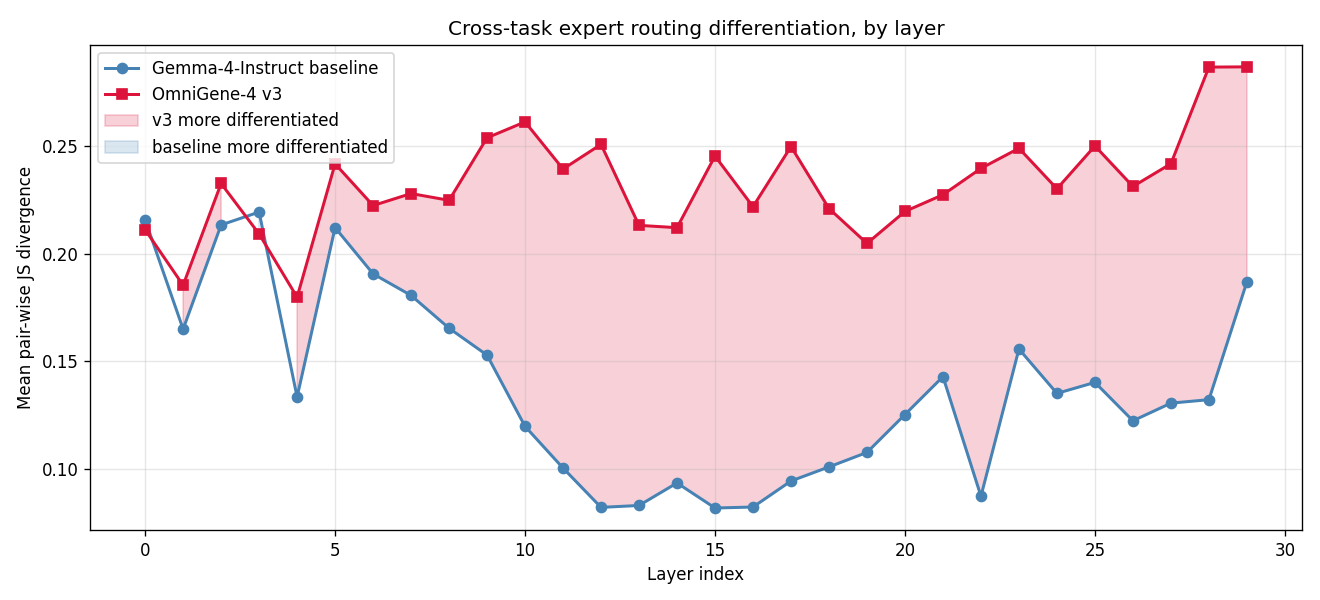
\includegraphics[width=0.95\linewidth]{figures/fig3_per_layer_js.png}
\caption{Per-layer mean pair-wise JS divergence across 8 task pools. Red: OmniGene-4 v3; blue: Gemma-4-Instruct baseline.}
\label{fig:per-layer-js}
\end{figure}

The differentiation is not concentrated in shallow embedding-proximal layers: the largest gains are at layer 12--28, i.e. in the semantic-processing depth of the network. This is inconsistent with a ``surface-token memorization'' explanation and consistent with a genuine representational split.

Per-task entropy analysis strengthens this conclusion. Under CPT+SFT training, Protein and DNA entropies \emph{decrease} (more concentrated expert use: Protein $2.76 \to 2.54$ nats, DNA $2.70 \to 2.53$), while NL entropy \emph{increases} ($3.85 \to 4.13$). Biological tasks converge onto dedicated experts; NL spreads across a wider but distinct set --- so the model is \emph{broadening} its linguistic capacity rather than narrowing it. This is a direct refutation of a catastrophic-forgetting narrative for this training recipe.

\subsubsection{Decomposition: CPT vs SFT}
\label{sec:moe-decomp}

Because we have all three checkpoints (baseline, cpt, v3), we can ask which stage produced the observed differentiation. Writing $\Delta_{\mathrm{CPT}}(\ell) = J_{\mathrm{cpt}}(\ell) - J_{\mathrm{baseline}}(\ell)$ and $\Delta_{\mathrm{SFT}}(\ell) = J_{\mathrm{v3}}(\ell) - J_{\mathrm{cpt}}(\ell)$ for the mean pair-wise JS at layer $\ell$:

\begin{table}[H]
\centering
\small
\caption{Stage-wise decomposition of cross-task routing differentiation.}
\label{tab:decomp}
\begin{tabular}{lrr}
\toprule
\textbf{Stage} & \textbf{Avg JS across layers} & \textbf{$\Delta$} \\
\midrule
Baseline                         & $0.1383$ & ---       \\
$+\,$ CPT 0.6-epoch              & $0.2304$ & $\mathbf{+0.0921}$ (98\%) \\
$+\,$ SFT $+$ 20K remote (v3)    & $0.2323$ & $+0.0019$ (2\%) \\
\bottomrule
\end{tabular}
\end{table}

\textbf{Nearly the entire expert-differentiation effect is produced by CPT.} SFT contributes essentially nothing to the routing-divergence metric. The per-layer decomposition (Figure~\ref{fig:decomp}) is even more striking: CPT adds mass in middle layers ($L_{11}$--$L_{27}$, peak $+0.16$ at $L_{12}$); SFT adds mass almost exclusively at the final two layers ($L_{28}$, $L_{29}$), peak $+0.048$ at $L_{29}$.

\begin{figure}[H]
\centering
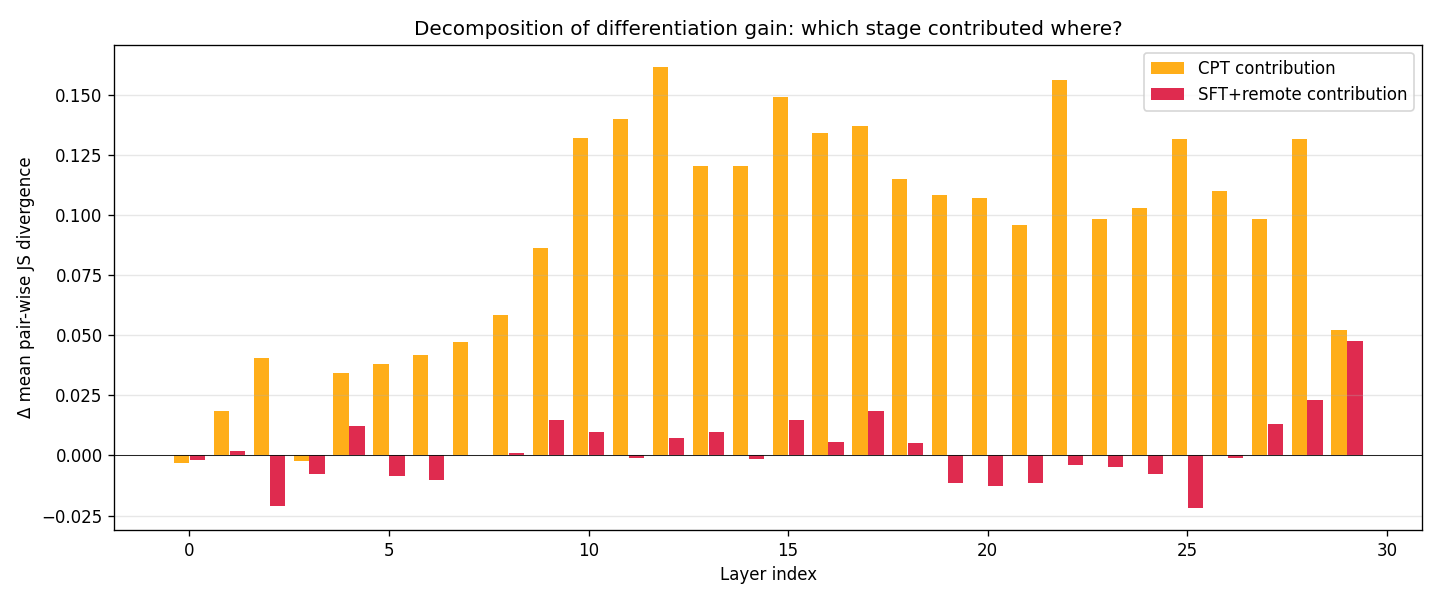
\includegraphics[width=0.95\linewidth]{figures/fig4_js_decomposition.png}
\caption{Per-layer decomposition of cross-task JS gain. Orange: CPT-stage contribution; red: SFT-stage contribution. CPT drives middle-layer representation differentiation; SFT drives final-layer output alignment.}
\label{fig:decomp}
\end{figure}

This gives a clean interpretation of the two training stages:
\begin{itemize}\setlength\itemsep{2pt}
\item \textbf{CPT = representation differentiation.} The router learns ``this token is DNA / NL / Cell / \ldots'' in the middle layers. No task-specific formatting is required: unlabeled next-token prediction on mixed corpora is sufficient.
\item \textbf{SFT = output alignment.} At the layers adjacent to \texttt{lm\_head}, SFT teaches the model ``when the user asks for homology, emit \texttt{Homologous} or \texttt{Non-Homologous}''. No new representation is created; existing experts are re-weighted to bias generation.
\end{itemize}

The correspondence to benchmarks is immediate: Standard-homology accuracy (100\%) comes from SFT (representation existed after CPT, SFT aligned output); Remote-homology accuracy (60\%) is bounded by CPT's representational split, and adding 20K remote pairs at SFT moves the needle only $+3$ points because representation is frozen.

\subsubsection{Per-task isolation and global heatmap}
\label{sec:moe-isolation}

Figure~\ref{fig:heatmap-delta} shows the task $\times$ expert difference in routing probability (v3 minus baseline), layer-averaged. Red indicates experts more used by v3; blue more used by baseline. The NL row shows bidirectional extremes (some experts vacated, new specialized ones recruited), Cell and Mol share their newly recruited experts (E6, E97, E100), and the RemHomology row introduces a distinct set of protein-character experts (E48, E72, E110, E114, E115).

\begin{figure}[H]
\centering
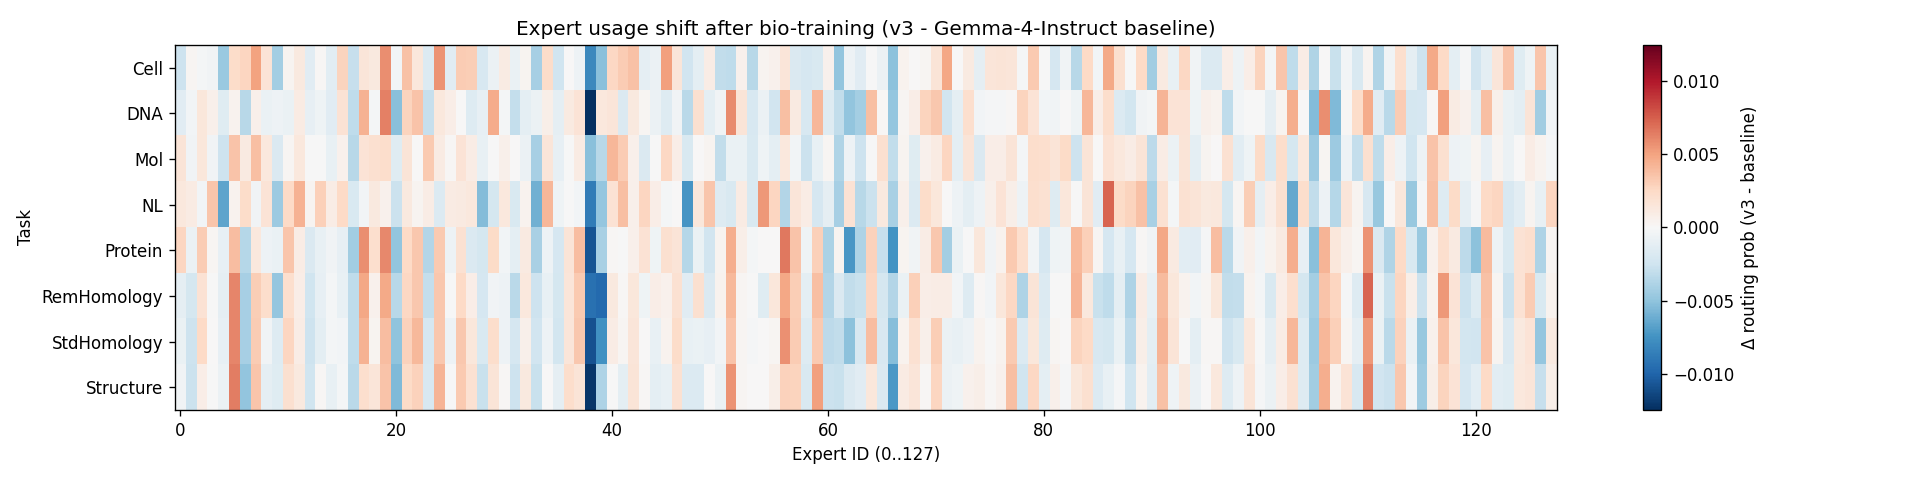
\includegraphics[width=0.95\linewidth]{figures/fig2_heatmap_delta.png}
\caption{Layer-averaged $\Delta$ routing probability (v3 $-$ baseline) across 8 tasks. Red: more used after training; blue: less used.}
\label{fig:heatmap-delta}
\end{figure}

\begin{table}[H]
\centering
\small
\caption{Per-task average JS-to-other-tasks (all layers).}
\label{tab:isolation}
\begin{tabular}{lrrrrr}
\toprule
\textbf{Task} & \textbf{Baseline} & \textbf{CPT} & \textbf{v3} & \textbf{$\Delta$ CPT} & \textbf{$\Delta$ SFT} \\
\midrule
NL           & 0.255 & 0.442 & 0.436 & $\mathbf{+0.187}$ & $-0.006$ \\
Cell         & 0.140 & 0.268 & 0.270 & $\mathbf{+0.128}$ & $+0.002$ \\
Mol          & 0.144 & 0.233 & 0.244 & $+0.089$ & $+0.010$ \\
DNA          & 0.144 & 0.226 & 0.224 & $+0.082$ & $-0.002$ \\
Protein      & 0.117 & 0.193 & 0.198 & $+0.076$ & $+0.005$ \\
StdHomology  & 0.101 & 0.162 & 0.163 & $+0.061$ & $+0.000$ \\
RemHomology  & 0.108 & 0.168 & 0.173 & $+0.060$ & $+0.005$ \\
Structure    & 0.097 & 0.150 & 0.151 & $+0.053$ & $+0.001$ \\
\bottomrule
\end{tabular}
\end{table}

NL's isolation grows the most ($+0.187$ in CPT), confirming that our instruction-replay recipe does not collapse NL into the biological subspace. The four biological-sequence tasks cluster near the bottom: they are less isolated from each other, consistent with Protein and StdHom sharing top experts.

\section{Discussion}
\label{sec:discussion}

\subsection{Representation vs alignment: a training-stage factorization}

The 98\% / 2\% split between CPT and SFT contributions to expert differentiation is, to our knowledge, the first direct measurement of its kind in a biological MoE. It complements recent empirical work on CPT/SFT balance in general LLMs \citep{ibrahim2024cpt, jindal2024balance} and on fine-grained expert specialization \citep{dai2024deepseekmoe}, extending these findings into the biological domain. It suggests that the two stages of post-pretraining are doing qualitatively different things rather than two sizes of the same thing. CPT performs \emph{representation differentiation}: it teaches the router which tokens belong to which modality. This happens in the middle transformer layers ($L_{11}$--$L_{22}$) and is the slow, expensive, data-hungry phase. SFT performs \emph{output alignment}: at the layers adjacent to \texttt{lm\_head}, it re-weights the final routing decisions so the model produces correctly-formatted answers. It does not meaningfully alter the model's internal representations.

This reframing has immediate practical consequences. When a practitioner observes a disappointing result --- for example, our 60\% remote-homology accuracy --- the conventional response is to add more labeled examples for that task. Our measurements suggest this response is misdirected. The router has already partitioned proteins into a shared expert pool; remote-homology identification is a \emph{mixture-weight} problem over that fixed pool, and SFT has limited leverage on mixture weights from a few hundred thousand examples. The correct response is to enrich CPT with more distant-protein pairs.

\subsection{Catastrophic forgetting is avoidable, but the mechanism matters}

In our earlier v1 experiments with LLaMA-3.1 8B + Bio-SFT (no instruction replay), BixBench dropped by 17 points (80\% $\to$ 63\%), matching the forgetting pattern documented in \citep{luo2023forgetting, huang2024sssr}. In the present v3, with 20\% OpenWebText \citep{gadre2021pile} in the CPT mixture and $\sim 20\%$ instruction replay in the SFT pool, BixBench rises by 6.7 points relative to Gemma-4-Instruct. The router-level analysis explains why. Natural-language tokens in v3 are routed to a \emph{different} set of experts after CPT (NL entropy rises from 3.85 to 4.13 nats --- the router uses \emph{more} experts for NL, not fewer), while biological tokens concentrate on a \emph{narrower} set (Protein entropy falls from 2.76 to 2.54 nats). The two populations essentially occupy disjoint corners of expert-space. Catastrophic forgetting in dense models can be thought of as the new training signal overwriting the old; in MoE it instead manifests as one population displacing another from a shared expert pool. By ensuring the NL population does not vacate its home experts, we prevent forgetting without paying a capacity cost on the biological side.

\subsection{Interpretability dividends of MoE}

The five atomic experts we identify (E54 English function-word, E59/E117 DNA dinucleotide, E78 amino-acid, E97 cellular-biology) are individually modest findings --- each explains perhaps 1--2\% of the model's compute at its home layer. But collectively they vindicate a methodological claim rarely demonstrated for bio-foundation models: \emph{MoE routing can be read off as an explicit, auditable specification of which subnetwork processes which input}. This is a different interpretability substrate from sparse-autoencoder features \citep{templeton2024scaling, bricken2023monosemanticity} or attention-based probing \citep{adams2025scfminterp}: it requires no classifier fitted on hidden states and no dictionary learned over activations. The English function-word expert, at 80\% purity on \texttt{the}, \texttt{.}, \texttt{,}, is sharp enough to be verified by a curious user on any new dataset.

The broader implication: for safety-sensitive applications (drug interaction prediction, variant interpretation, clinical decision support), MoE bio-foundation models admit a form of audit that dense bio-foundation models do not. If the model classifies a novel protein variant as ``pathogenic'', one can check \emph{which experts it used} and \emph{on which residues those experts fired}. We did not pursue this line of inquiry here, but the infrastructure developed in \S\ref{sec:hooks} supports it directly.

\subsection{Relation to other bio-foundation models}

Our 99.95\% standard-homology and 59.50\% remote-homology accuracies place OmniGene-4 in competitive territory. Specialist models \citep{lin2023evolutionary, elnaggar2021prottrans, hamamsy2024protein, liu2024plmsearch} achieve slightly higher remote accuracy (65--75\%) but without the cross-modal and natural-language capabilities our model exhibits simultaneously. Unified DNA/protein models such as LucaOne \citep{he2024lucaone} and genome-scale models such as Evo \citep{nguyen2024evo, brixi2026evo2} pursue different design tradeoffs, focusing on sequence generation rather than instruction-following. Qwen-3 has been reported at $\approx 75\%$ on remote homology but at an order of magnitude more active parameters and, as far as we know, without router-level analysis. The present paper's contribution is less about the benchmark ceiling than about the methodological surface area: we provide a quantitatively reproducible decomposition of what CPT and SFT each contribute, which may generalize to other MoE bio-foundation efforts.

\section{Limitations and future work}
\label{sec:limitations}

\paragraph{Top-1 expert purity is modest.} The highest-purity atomic expert we identified (E54, English function-words) reaches 80\%, but most ``specialty'' experts land at 15--35\% purity. Our claims about task-specific experts should be understood distributionally rather than as hard assignments.

\paragraph{Single model family.} All results are from Gemma-4-26B-A4B-Instruct. Whether the 98\%/2\% CPT/SFT decomposition generalizes to Mixtral \citep{jiang2024mixtral}, DeepSeek-MoE, or GPT-class bio models is an open question. The architectures differ in expert count, top-$k$ selection, and router objective.

\paragraph{Remote-homology ceiling.} Our 60\% remote-homology accuracy is well below specialist models (ESM-2 \citep{lin2023evolutionary} at $\approx 75\%$). We hypothesized this is a representation-level constraint rather than an SFT-scale constraint; testing requires controlled experiments with more CPT on distant-protein pairs. This was estimated at $\approx 150$ GPU-hours and is deferred to future work.

\paragraph{No chain-of-thought reasoning.} We briefly attempted to train with \texttt{<THOUGHT>} reasoning blocks for remote homology but abandoned it because synthetic-CoT templates from sequence features were of insufficient quality. Human-expert or strong-teacher-generated CoT data would likely improve remote-homology performance substantially.

\paragraph{Evaluation scale.} BixBench's True/False subset contains only $\approx 200$ questions; small absolute differences in the 90--95\% range are within the dataset's noise floor. Richer evaluation pools (HELM-Bio, LM-BIO) would strengthen the claims.

\subsection*{Future experiments}

Based on the decomposition results, we propose three concrete follow-ups: \emph{(1)} a CPT-scaling study on 100\,GB of curated distant-protein pairs from SCOP \citep{murzin1995scop} or CATH fold-level annotations to test whether the representation-level bottleneck for remote homology is relieved; \emph{(2)} packaging the forward-hook infrastructure (\S\ref{sec:hooks}) as a reproducible command-line router-audit tool for bioinformatics practitioners; \emph{(3)} cross-architecture replication on Mixtral-8x7B or DeepSeek-MoE bio variants to test whether the 98\%/2\% split is a property of MoE training generally.

\subsection*{Code and data availability}

All training scripts (\texttt{biopaws/cpt/1-prepare\_cpt\_data\_mp.py}, \texttt{biopaws/cpt/2-run\_cpt.py}, \texttt{biopaws/sft\_data/14-train\_bio\_sft\_v2.py}, \texttt{biopaws/sft\_data/17-train\_bio\_sft\_v3\_remote.py}), evaluation scripts, and analysis scripts (\texttt{biopaws/cpt/20--24*.py}) are available in the project repository. The token-level activation database and routing-count matrices are in \texttt{outputs/moe\_analysis/}. LoRA adapter weights and embedding checkpoints ($\approx 1.9$\,GB) can be released on reasonable request.

\bibliographystyle{plainnat}
\bibliography{refs}

\end{document}
